\chapter{Erstellung von Kookkurrenzgraphen}

\section{MapReduce}
\label{mapreduce}

MapReduce \cite{dg2004} ist ein Programmiermodell für nebenläufige Verarbeitung und Erzeugung großer Datenmengen. Der Grundgedanke dieses Modells besteht in der Zerlegung der Berechnung in zwei Funktionen: \emph{Map} und \emph{Reduce}. Die Ein- und Ausgabedaten sind Schlüssel-/Wertpaare. Beide Funktionen werden vom Benutzer spezifiziert.

Die Map-Funktion dient zur Erzeugung von Zwischenergebnissen, ebenfalls in der Form von Schlüssel-/Wertpaaren. Die Funktion wird einzeln auf jedes Paar der Eingabedaten angewandt und kann eine beliebige Anzahl von Zwischenergebnissen \emph{emittieren}. Die MapReduce-Bibliothek gruppiert daraufhin alle Paare mit dem gleichen Schlüssel und übergibt diese an die Reduce-Funktion.

Die Reduce-Funktion wird also jeweils auf einen Schlüssel und eine Liste von Werten angewandt. Ziel dieser Funktion ist, für jeden Schlüssel kein oder ein Ergebnis zurückzugeben. Die zu reduzierenden Werte werden für gewöhnlich als Iterator übergeben, um auch Datenmengen verarbeiten zu können, die nicht in den Arbeitsspeicher des Rechenknotens passen. Die Reduce-Funktion wird nur angewandt, wenn nach dem Map-Schritt mehr als ein Wert für einen Schlüssel emittiert wurde. Somit sollten Map- und Reduce-Funktion das gleiche Ausgabeformat besitzen. Das grundsätzliche Vorgehen von MapReduce ist in Abbildung \ref{fig:mapreduce} abgebildet.

\begin{figure}
\centering
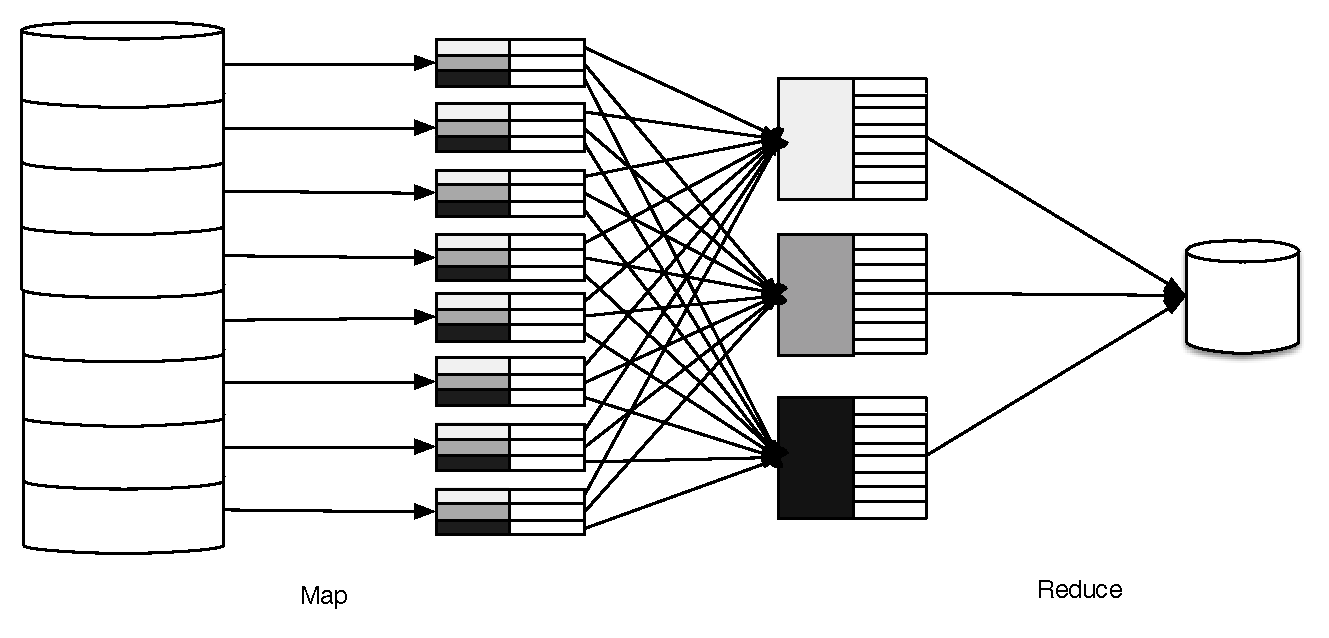
\includegraphics[width=\textwidth]{mapreduce}
\caption{MapReduce-Prozess}
\label{fig:mapreduce}
\end{figure}

Die MapReduce-Bibliothek übernimmt sämtliche Kommunikation zwischen den Knoten des Rechnerclusters. Dies hat den Vorteil, dass sich der Programmierer nur über die Umwandlung des zu lösenden Problems auf das Programmiermodell, nicht aber um dessen Implementierung über mehrere Rechner hinweg kümmern muss. Somit kann die verwendete Hardware vergleichsweise einfach an die zu verarbeitende Datenmenge oder die Bedürfnisse an die Rechengeschwindigkeit angepasst werden.

In dieser Arbeit wurde die MapReduce Implementierung von MongoDB eingesetzt (siehe \ref{mongo}). Nach dieser grundsätzlichen Betrachtung des Programmiermodelles wird im nächsten Abschnitt die Anwendung zur Berechnung von Konkurrenzen diskutiert.

\section{Anwendung von MapReduce zur Kookkurrenzberechnung}
\label{mapreduce_cooccurence}

MapReduce kann für die Berechnung der Knoten und Kanten des Kookkurrenzgraphen genutzt werden. Dazu müssen für beide Operationen das Ein- und Ausgabeformat sowie die Funktionen Map und Reduce definiert werden.

Um die Berechnung zu vereinfachen, werden zuerst die Knoten erzeugt und mit allen Vorkommen der Begriffe annotiert. Somit kann daraufhin direkt aus der Knotenmenge die Kantenmenge erzeugt werden. Außerdem werden bei der Nutzung der Daten weniger Anfragen benötigt, um Informationen über einen Begriff selbst zu bekommen.

\subsection{Berechnung der Knoten}

Als Eingabedaten für die Berechnung der Knotenmenge dienen Tupel der Form \((d, t)\), wobei \(d\) ein Dokument und \(t\) einen Begriff darstellt. Die Map-Funktion wird nun auf jeden dieser Tupel angewandt und emittiert Schlüssel-/Wertpaare mit dem Begriff als Schlüssel und einer einelementigen Liste, die das Dokument des Tupels enthält sowie der Zahl \num{1} als Anzahl Vorkommen dieses Begriffs. Dieses Vorgehen ist notwendig, da die Ausgabe der Map- und Reduce-Funktionen das gleiche Datenformat haben sollten.

Die Reduce-Funktion fasst die einelementigen Listen zusammen, addiert die Vorkommen und erzeugt somit den Knoten, der für einen Begriff alle Dokumente, die mit diesem Begriff versehen wurden, sowie die Anzahl der Vorkommen insgesamt enthält.

Die Map- und Reduce-Funktionen für die Knotenberechnung sind in Listings \ref{lst:mapred_nodes} als Pseudo--Code dargestellt.

\begin{lstlisting}[language=pseudo, label={lst:mapred_nodes}, caption={Knotenerzeugung mit MapReduce}]
function map(document, term) {
    emit(term, {documents: [document], count: 1});
}

function reduce(term, values) {
    result = {documents: [], count: 0};
    foreach value in values do
        result.documents = concat(result.documents, value.documents);
        result.count = result.count + value.count;
    end
    return result;
}
\end{lstlisting}

\subsection{Berechnung der Kanten}

Die Berechnung der Kantenmenge kann mit den vorher berechneten Knoten als Eingabedaten erfolgen und wird in 2 Verarbeitungsschritte aufgeteilt. Zuerst werden die annotierten Knoten so umgeformt, dass zu einem Dokument alle vergebenen Begriffe bekannt sind. Im zweiten Schritt werden alle Paare von miteinander auftretenden Begriffen gebildet und die Ähnlichkeitsmaße berechnet.

Algorithmus \ref{lst:mapred_edges1} zeigt die Umformung der Knoten mittels MapReduce. Als Eingabe für die Map-Funktion dienen die Knoten. Diese werden so umgeformt, dass für jedes Dokument, das am Knoten annotiert ist, ein neues Schlüssel-/Wertpaar emittiert wird. Die Reduce-Funktion fasst die emittierten Ergebnisse zusammen, sodass als Ergebnis alle Begriffe, die an ein Dokument vergeben wurden, gesammelt als Liste vorliegen.

\begin{lstlisting}[language=pseudo, label={lst:mapred_edges1}, caption={Umformung der Knoten mit MapReduce}]
function map(node) {
    foreach document in node.documents do
        emit(document, {terms: [node]});
    end
}

function reduce(term, values) {
    result = {terms: []};
    foreach value in values do
        result.terms = concat(result.terms, value.terms);
    end
    return result;
}
\end{lstlisting}

In Algorithmus \ref{lst:mapred_edges2} wird die Erzeugung der Kookkurrenzkanten dargestellt. Im Map-Schritt werden dazu alle möglichen Paare der mit einem Dokument verknüpften Begriffe gebildet und emittiert. Der Schlüssel ist eine Kombination aus Ziel- und Quellbegriff. Der Wert zählt die Anzahl der Kookkurrenzen zwischen beiden Begriffen. Im Reduce-Schritt werden alle Kanten zwischen zwei Termen zusammengefasst, die Summe der Kookkurrenzen gebildet und die Ähnlichkeitsmaße berechnet. Die Funktionen zur Berechnung der Maße sind in \ref{measures} beschrieben.

\begin{lstlisting}[language=pseudo, label={lst:mapred_edges2}, caption={Kantenerzeugung mit MapReduce}]
function map(document) {
    foreach term1 in document.terms do
        foreach term2 in document.terms do
            emit({source: term1, target: term2}, {count: 1});
        end
    end
}

function reduce(edge, values) {
    result = {count: 0, dice: 0, jaccard: 0, cosine: 0};
    foreach value in values do
        result.count = result.count + value.count;
    end
    result.dice = dice(edge.source, edge.target, result.count);
    result.jaccard = jaccard(edge.source, edge.target, result.count);
    result.cosine = cosine(edge.source, edge.target, result.count);
    return result;
}
\end{lstlisting}

Nachdem in diesem Kapitel die theoretischen Grundlagen für die Link Discovery mittels Kookkurrenz beschrieben wurden, beschäftigt sich das folgende Kapitel mit dem technischen System zur Umsetzung des Lösungsansatzes.